This chapter reports the experimental outcomes for both training performance on the synthetic dataset and generalization to real instruments using NSynth. The results are grouped into training behavior, parameter prediction accuracy, and audio similarity metrics.

\section{Training Results}

Table~\ref{tab:train_val_metrics_2} summarizes the last five epochs of training, showing stable convergence and no signs of overfitting. Figure~\ref{fig:mae_mse_evolution} illustrates the evolution of MAE and MSE across epochs.

\begin{table}[htb]
  \centering
  \small
  \caption{Training and validation metrics by epoch.}
  \label{tab:train_val_metrics_2}
  \begin{tabular}{c|ccc|ccc}
    \hline
    Epoch & \multicolumn{3}{c|}{Train} & \multicolumn{3}{c}{Validation} \\
     & Loss & MAE & MSE & Loss & MAE & MSE \\
    \hline
    70 & 0.603 & 0.527 & 0.545 & 0.622 & 0.517 & 0.562 \\
    71 & 0.601 & 0.526 & 0.542 & 0.637 & 0.520 & 0.569 \\
    72 & 0.605 & 0.526 & 0.545 & 0.621 & 0.516 & 0.565 \\
    73 & 0.602 & 0.524 & 0.541 & 0.625 & 0.522 & 0.568 \\
    74 & 0.611 & 0.528 & 0.548 & 0.625 & 0.520 & 0.563 \\
    \hline
  \end{tabular}
\end{table}

\begin{figure}[h]
    \centering
    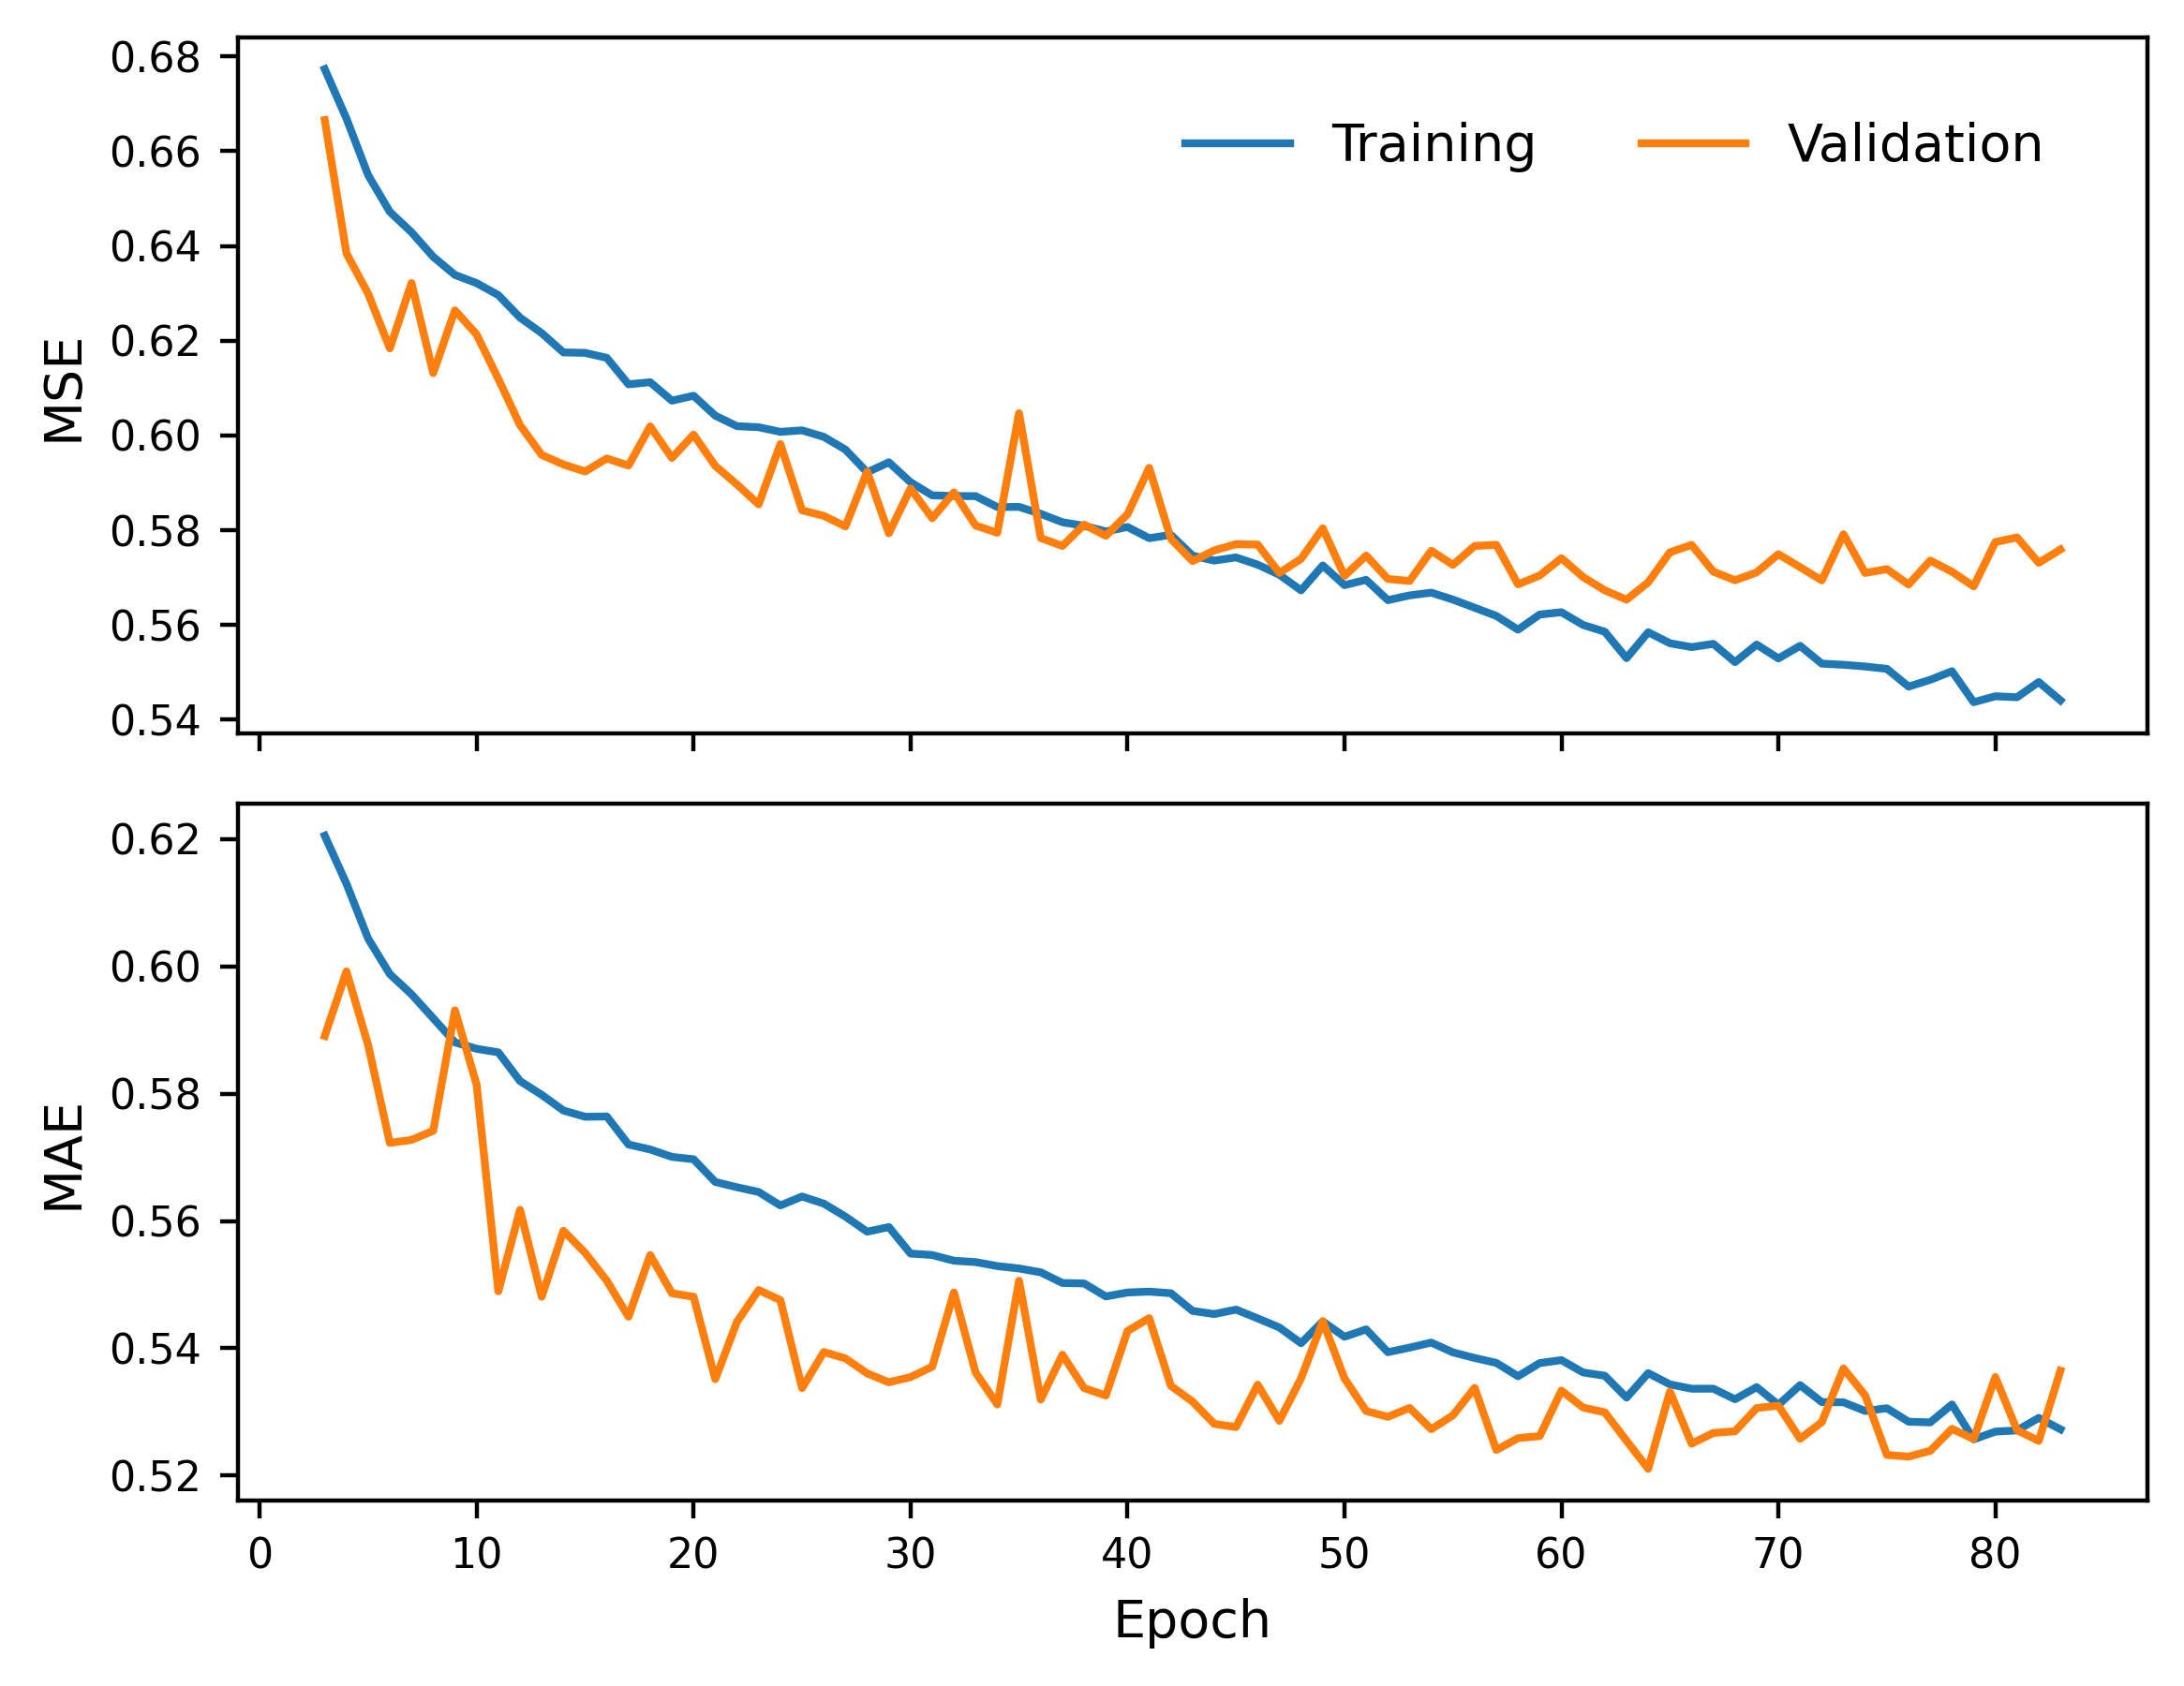
\includegraphics[width=\linewidth]{../images/mae_mse_evolution.png}
    \caption{Evolution of MAE and MSE during training.}
    \label{fig:mae_mse_evolution}
\end{figure}

After training, a held-out synthetic split was used to compute test errors in the original parameter space. The results were:

\begin{itemize}
\item Mean Absolute Error (MAE): 6.488
\item Mean Squared Error (MSE): 1410.097
\item Root Mean Squared Error (RMSE): 37.551
\end{itemize}

\section{Audio Comparison Results}

Generalization was evaluated by re-synthesizing the NSynth test set and comparing the generated audio against the original recordings. A baseline comparison was computed using a pure 440 Hz sinusoid. Table~\ref{tab:metrics} shows mean and standard deviation values, and the improvement is defined as \((\text{baseline} - \text{resynthesis}) / \text{baseline}\).

\begin{table}[htb]
  \centering
  \small
  \caption{Resynthesis vs. baseline with improvement (mean and standard deviation in parentheses).}
  \label{tab:metrics}
  \begin{tabular}{l|c|c|c|c}
    \hline
    & FFT & STFT & Log Mel (raw) & Log Mel (normalized) \\
    \hline
    Resynthesis & 12649.9 (6208.1) & 2366.4 (1132.2) & 138.73 (47.013) & 0.0086 (0.0029) \\
    Baseline & 33508.8 (1887.36) & 7290.4 (434.87) & 184.87 (30.136) & 0.0115 (0.0019) \\
    Improvement (\%) & 62.250 & 67.540 & 24.960 & 24.930 \\
    \hline
  \end{tabular}
\end{table}

To analyze behavior across timbral families, metrics were aggregated by instrument group. Table~\ref{tab:avg_metrics_groups} presents the average values. The best results were obtained for keyboard, guitar, and mallet families, while vocal and organ were the most challenging.

\begin{table}[htb]
  \centering
  \small
  \caption{Average values by instrument group.}
  \label{tab:avg_metrics_groups}
  \begin{tabular}{l|c|c|c|c}
    \hline
    Group & FFT & STFT & Log Mel (raw) & Log Mel (normalized) \\
    \hline
    bass     & 11232.7 & 2144.32 & 135.610 & 0.00841 \\
    brass    & 14371.1 & 2682.95 & 167.617 & 0.01039 \\
    flute    & 14611.3 & 2872.69 & 141.819 & 0.00879 \\
    guitar   & 9692.0  & 1867.47 & 119.853 & 0.00743 \\
    keyboard & 9619.3  & 1772.92 & 119.529 & 0.00741 \\
    mallet   & 8085.8  & 1632.45 & 120.610 & 0.00748 \\
    organ    & 18360.1 & 3453.13 & 166.433 & 0.01032 \\
    reed     & 12740.0 & 2267.08 & 140.701 & 0.00872 \\
    string   & 12883.7 & 2390.65 & 139.365 & 0.00864 \\
    vocal    & 31028.9 & 5271.26 & 212.646 & 0.01319 \\
    \hline
  \end{tabular}
\end{table}

\section{Discussion}

The training curves indicate stable convergence with small gaps between training and validation losses, suggesting good generalization for the synthetic domain. The parameter prediction errors are consistent with the expected variability of the FM parameter space.

In the NSynth evaluation, the model consistently outperformed the sinusoidal baseline across all metrics, with the largest gains observed in FFT and STFT distances. The Log-Mel improvements are smaller but still substantial, indicating a closer perceptual match. Differences across instrument families highlight that timbres with more complex spectral envelopes (e.g., vocal, organ) remain more challenging, whereas harmonic-rich but structured families (e.g., keyboard, guitar, mallet) are better captured.
